En esta sección se ofrece una revisión de los componentes de un motor \ac{DC} y su respectivo modelo matemático. Además, se examinarán los métodos y algoritmos más comunes en la estimación de parámetros. Dicha información será utilizada para el desarrollo de algoritmos orientados a la estimación de los parámetros característicos de los motores \ac{DC}.
    \section{Introducción}
    \label{sec:CH02_INTRODUCCION}
    A continuación se resumirán las partes que conforman un motor de corriente continua, tomando de referencia al libro ``Modelado y simulación de sistemas dinámicos'' escrito por \textcite{libro_aleman}.\\
    %``texto''-> para abrir las comillas
    Los motores \ac{DC} son actuadores que convierten la energía eléctrica en mecánica con el propósito de generar un movimiento rotatorio. Se componen principalmente de dos estructuras magnéticas: el rotor y el estator. De esas 2 estructuras mencionadas, se logran identificar más componentes que influirán en la dinámica de un motor; estos se muestran en forma de esquema en la Figura~\ref{fig:subfig1} y como componentes físicos en la Figura~\ref{fig:subfig2}. 
    \begin{figure}[!ht]
    \begin{tabularx}{\linewidth}{*{2}{>{\centering\arraybackslash}X}}
        % FILA-1, COL-1 (imagen izquierda)
        \begin{subfigure}[t]{0.45\textwidth}
            \centering
            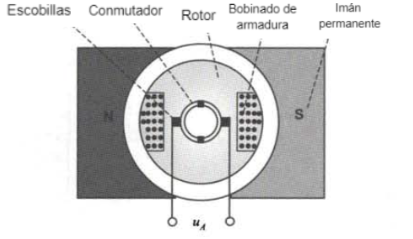
\includegraphics[width=.9\linewidth]{ANNEX/Fig/AC/AC_02_PartesDeMotor2.PNG}
        \end{subfigure}
        &
        % FILA-1, COL-2 (imagen derecha)
        \begin{subfigure}[t]{0.45\textwidth}
            \centering
            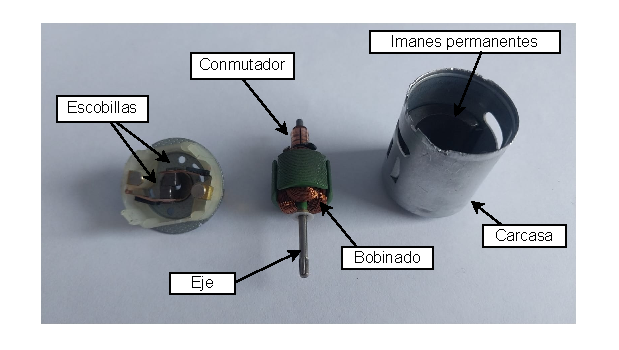
\includegraphics[width=.9\linewidth]{ANNEX/Fig/AC/AC_03_PartesDeMotor3.pdf}
        \end{subfigure}
        \\
        % FILA-2 (captions individuales)
        \begin{subfigure}[t]{0.8\linewidth}
            \caption{Esquema de un motor \ac{DC} de imán permanente}
            \label{fig:subfig1}
        \end{subfigure}
        &
        \begin{subfigure}[t]{0.8\linewidth}
            \caption{Componentes que conforman un motor \ac{DC} 6V}
            \label{fig:subfig2}
        \end{subfigure}
        \\
        % FILA-3 (notas)
        \begin{subfigure}[t]{\linewidth}
            \caption*{\textit{Nota: Figura adaptada de \textcite{libro_aleman}}}
        \end{subfigure}
        &
        \begin{subfigure}[t]{\linewidth}
            \caption*{} % Sin nota para la subfigura derecha
        \end{subfigure}
    \end{tabularx}
    \caption{Identificación de las piezas que forman un motor \ac{DC}}
    \label{fig:figura_con_subfiguras}
\end{figure}

    En un motor de corriente continua con imanes permanentes, el campo magnético es generado por los propios imanes que se encuentran en el estator, mientras que el rotor, aquel que contiene el bobinado, gira dentro de dicho campo magnético. La tensión será aplicada directamente por las escobillas y el encargado de mantener la correcta dirección de la corriente será el conmutador para permitir la generación de par. \autocite{libro_aleman}. 
    \section{Modelo lineal de un motor \ac{DC}}
    \label{sec:CH02_ModeloMDC}
    Si se desea controlar este tipo de motores, es importante conocer las consideraciones y aproximaciones matemáticas que describen su dinámica. A continuación, se presenta un esquema electromecánico como punto de partida para modelar el sistema.
    La velocidad angular $\omega(t)$ está controlada por el voltaje de entrada $u(t)$, con una caída de voltaje constante atribuida a la resistencia de las escobillas y del rotor, y una \ac{FEM} $u_a(t)$ causada por la armadura giratoria.
    La inductancia $L$ del motor contribuye proporcionalmente al cambio en la corriente del motor $i(t)$. La corriente del motor acopla el componente eléctrico con el mecánico, ya que genera el par motor $\tau(t)$. Este par se ve antagonizado por la inercia del motor $J$, la amortiguación de la estructura, el torque generado por la fricción $T_v$ y la carga externa $T_L$ (M. Ruderman et al., 2018). Este trabajo de investigación se centrará en hallar los valores de las constantes que permitan modelar un motor \ac{DC}; las variables a hallar son la resistencia $R$, la inductancia del motor $L$, la inercia del motor $J$, el coeficiente de fricción viscosa $\mu$ y las constantes $k_e$ y $k_t$, que relacionan, a la velocidad angular $\omega(t)$ con el voltaje de la \ac{FEM} $u_a(t)$,  la corriente $i(t)$ con el torque del motor $\tau(t)$ y la fricción $\mu$ con el torque $T_v$ generado por esta, respectivamente. A partir de la Figura~\ref{fig:esquema}, se puede describir la dinámica de un motor de corriente continua aplicando las leyes de Kirchhoff para analizar el circuito eléctrico y la segunda ley de Newton para modelar el movimiento del rotor. A continuación, se presentan ambas ecuaciones:\\
    \begin{minipage}{0.60\textwidth}
    %\vspaceTextToFigure % =\vspace{0.1cm}}\
        \centering 
        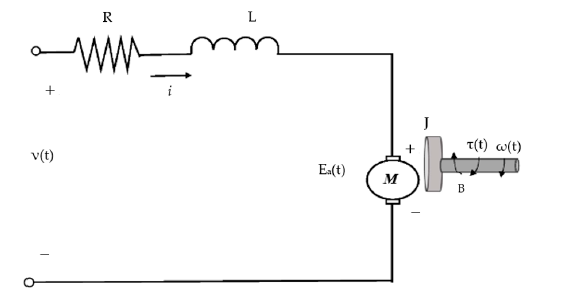
\includegraphics[width=0.8\textwidth]{ANNEX/Fig/AC/AC_04_ModeladoDeMotor.PNG}
        \captionof{figure}{Diagrama electromecánico de un motor de corriente continua \autocite{Electronics}}
        \label{fig:esquema}      
    \end{minipage}
    \begin{minipage}{0.40\textwidth}
    %\vspaceTextToFigure % =\vspace{0.1cm}
    \begin{align}
        u(t) = i(t)R + L\frac{di}{dt} + u_a(t) 
        \\\tau(t) = J\frac{d\omega(t)}{dt} + T_v + T_L,
    \end{align}
    \end{minipage}
    %conitnua texto
    \\
    de estas ecuaciones se puede definir 3 constantes de proporcionalidad: $k_t$, $k_e$ y $\mu$. Las 2 primeras han sido mencionadas anteriormente, y sirven para relacionar las variables eléctricas y mecánicas del sistema en el tiempo. En cuanto a la constante $\mu$, relaciona la velocidad angular $\omega$ con la fricción viscosa debido a que, a medida que la velocidad angular del rotor aumenta, las partículas de fluidos o los elementos de contacto generan una mayor fuerza de arrastre. En altas velocidades, este tipo de fricción es la dominante, mientras que en bajas velocidades predominan otras formas como la fricción estática y la fricción de Coulomb \autocite{friccion_marco_t}.
    Con lo antes mencionado, en este trabajo se consideran las siguientes relaciones lineales:
    \begin{equation}
        %\begin{gather}
        u_a(t) = K_e\,\omega(t), \quad
        \tau(t) = K_t\,i(t), \quad  
        T_v(t) = \mu\,\omega(t),
        %\end{gather}
        \label{eq:CH02_Relaciones_lineales}
    \end{equation}
    finalmente se puede expresar las ecuaciones diferenciales que describen el modelo de un motor \ac{DC} de la siguiente manera:
    \begin{align}
        u(t) = i(t)\,R + L\frac{di}{dt} + K_e\,\omega(t)
        \label{eq:ecu_electrica}\\[3pt]
        K_t\,i(t) = J\frac{d\omega(t)}{dt} + \mu\,\omega(t)
        \label{eq:ecu_mecanica}
    \end{align}

\subsection{Respuesta dinámica del sistema}
\label{sec:CH02_RespuestaMotor}
    La respuesta dinámica de un motor de corriente continua depende de su capacidad para ajustar la velocidad o el torque ante cambios en la entrada. Esto se determina por la constante de tiempo eléctrica, que mide la velocidad de respuesta del circuito a los cambios y está influenciada por la resistencia y la inductancia de los devanados, y la constante de tiempo mecánica, que mide el tiempo necesario para que el sistema mecánico responda y está afectada por la inercia del rotor, la carga y factores como la fricción o amortiguación \autocite{Electronics}.
    %La inercia del motor también influye en su dinámica: los motores con baja inercia reaccionan más rápido, mientras que los de alta inercia tardan más en estabilizarse.
    La dinámica de un motor de \ac{DC} puede dividirse en tres etapas: aceleración, estado estable y desaceleración, como se muestra en la Figura~\ref{fig:RPTA_DINAMICA}.
    \begin{figure}[H]
        \centering
        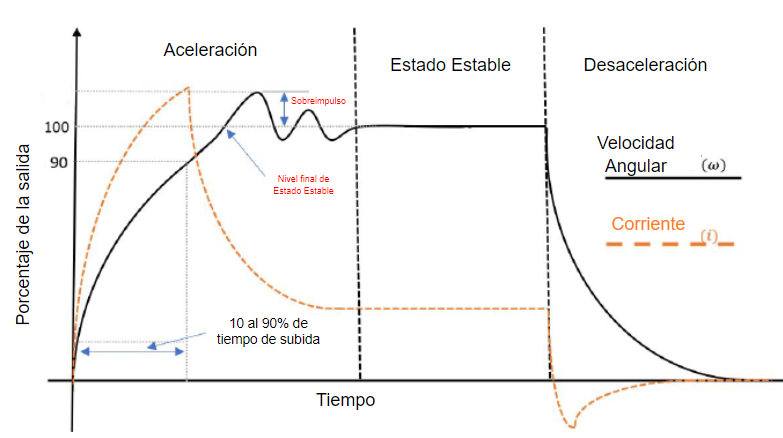
\includegraphics[width=0.8\textwidth]{ANNEX/Fig/AC/AC_05_ComportamientoDeMotor.PNG}
        \caption{Respuesta dinámica de un motor \ac{DC}. Adaptado de \autocite{Electronics}}
        \label{fig:RPTA_DINAMICA}
    \end{figure}  
       
\subsection{Representación en Espacio de Estados}
\label{sec:CH02_Representacion_MEE}
    La siguiente representación del modelo de un motor \ac{DC} fue consultada del libro “Modelado y control en espacio de estados” escrito por \textcite{MEE} distribuido por la Universidad Politécnica de Valencia.
    
    Para establecer un modelo matemático del sistema, en muchos casos puede considerarse un enfoque de caja negra, en el que no se conoce la naturaleza interna del mismo. Sin embargo, dado que en este trabajo se busca estimar parámetros físicos que representan con precisión el comportamiento real de un motor \ac{DC}, es necesario adoptar un enfoque más detallado, basado en su dinámica interna. Para ello, se requiere observar la evolución temporal de variables como la corriente $i(t)$, la velocidad angular $w(t)$ y el voltaje de entrada $u(t)$. Esta última puede omitirse como estado del sistema, ya que actúa como señal de entrada con la cual se excita al sistema durante el proceso de estimación.
  
    La representación interna o \ac{MEE}  permite analizar el estado interno del sistema en cada instante de tiempo. \textcite{MEE} define al estado como la información compactada de la actividad pasada que se ha tenido en el sistema, de forma que con esta información se puede predecir el comportamiento futuro del sistema ante una entrada cualquiera. 
    Para poder representar al sistema mediante \ac{MEE} serán necesarias 2 ecuaciones matriciales: la ecuación de estados y la ecuación de salida.
    Las técnicas de representación en el espacio de estado permiten describir sistemas de orden mayor mediante ecuaciones diferenciales de primer orden. En lugar de manejar una sola ecuación diferencial de $n$-ésimo orden, se utilizan $n$ ecuaciones de primer orden. Cada una de estas ecuaciones sigue una forma general, facilitando el análisis y control de sistemas complejos.
    \begin{align*}
        \frac{dx_i(t)}{dt} &= \sum_{j=1}^n a_{ij}\,x_j(t) + b_{i}\,u(t)\\
        y(t) &= \sum_{j=1}^n c_j\,x_j(t),
    \end{align*}
    si se desarrolla la expresión para $n$ variables de estado se tendrán expresiones de esta forma
    \begin{align*}
        \frac{dx_1(t)}{dt} &= \sum_{j=1}^n a_{1j}(t)\,x_j(t) + b_1\,u(t)= a_{11}\,x_1(t) + a_{12}\,x_2(t) + \cdots + a_{1n}\,x_n(t) + b_1\,u(t), \\
        \frac{dx_2(t)}{dt} &= \sum_{j=1}^n a_{2j}(t)\,x_j(t) + b_2\,u(t)= a_{21}\,x_1(t) + a_{22}\,x_2(t) + \cdots + a_{2n}\,x_n(t) + b_2\,u(t), \\
        &\vdots \\
        \frac{dx_n(t)}{dt} &= x_n(t) \sum_{j=1}^n a_{nj}(t)\,x_j(t) + b_n\,u(t) = a_{n1}\,x_1(t) + a_{n2}\,x_2(t) + \cdots + a_{nn}\,x_n(t) + b_n\,u(t),
    \end{align*}
    estas ecuaciones diferenciales pueden ser expresadas de forma matricial de  la siguiente manera: 
    \begin{align}
    \begin{bmatrix}
    \dot{x}_1(t) \\
    \dot{x}_2(t) \\
    \vdots \\
    \dot{x}_n(t)
    \end{bmatrix}
    &=
    \begin{bmatrix}
    a_{11} & a_{12} & \cdots & a_{1n} \\
    a_{21} & a_{22} & \cdots & a_{2n} \\
    \vdots & \vdots & \ddots & \vdots \\
    a_{n1} & a_{n2} & \cdots & a_{nn}
    \end{bmatrix}
    \begin{bmatrix}
    x_1(t) \\
    x_2(t) \\
    \vdots \\
    x_n(t)
    \end{bmatrix}
    +
    \begin{bmatrix}
    b_1 \\
    b_2 \\
    \vdots \\
    b_n
    \end{bmatrix}
    u(t)
    \label{eq:2.4}
    \\
    y(t) &=
    \begin{bmatrix}
    c_1 & c_2 & \cdots & c_n
    \end{bmatrix}
    \begin{bmatrix}
    x_1(t) \\
    x_2(t) \\
    \vdots \\
    x_n(t)
    \end{bmatrix}
    \label{eq:2.5}
    \end{align}
    Las ecuaciones anteriores pueden ser representadas de manera más compacta de la siguiente manera:\\
    \begin{align}
    	\dot{x}(t) &= A x(t) + B u(t), \label{eq:2.8}\\ 
    	y(t) &= C x(t) + D u(t), \label{eq:2.9}
   \end{align}
    
en donde:
\begin{itemize}
    \item $A \in\mbbb{n}{n}$ se le conoce como matriz de estado,
    \item $B \in\mbbb{n}{p} $ se le conoce como matriz de entrada,
    \item $C \in\mbbb{q}{n} $ se le conoce como matriz de salida,
    \item $D \in\mbbb{q}{p} $ se le conoce como matriz de ganancia directa.
\end{itemize}
La ecuación~\ref{eq:2.9}, conocida como la ecuación de estado del sistema, describe la evolución del estado en función de su valor actual y de la entrada. Además, algunas variables de estado pueden coincidir con las salidas, como se observa en la ecuación~\ref{eq:2.9}; esto se puede lograr cambiando el valor de los coeficientes de la matriz correspondiente al estado que se busca como salida $y$.
Las dimensiones de las matrices en el \ac{MEE} dependen de la cantidad de entradas, salidas y variables de estado que se definan. La dimensión $n$ estará determinada por el número de variables de estado, mientras que $p$ dependerá de la cantidad de entradas del sistema. En el caso de un motor \ac{DC}, se considera que como única entrada al voltaje $u(t)$, por lo tanto, se establece $p=1$. Por otro lado, la dimensión $q$ dependerá del número de salidas a definir. En este caso, se selecciona la velocidad angular $\omega(t)$ como la variable a controlar, dado que no cambia bruscamente como la corriente $i(t)$ y puede ser medida con instrumentos sencillos y económicos. A este tipo de sistemas se les conoce como \ac{SISO} porque cuenta con una única entrada y una única salida: $u(t)$ y $\omega(t)$, respectivamente. Sin embargo, también existen sistemas \ac{MIMO} , donde se manejan múltiples entradas y salidas, y la elección de \ac{SISO} o \ac{MIMO} depende del análisis del sistema y las variables que se busca controlar.

Algunos autores, como \textcite{MEE}, no incluyen el término D en la ecuación \ref{eq:2.9}. Esto tiene sentido si se busca la  representación de un motor \ac{DC}, ya que un valor no nulo de D implicaría que la salida responde instantáneamente a un cambio en el voltaje, lo cual contradice el comportamiento dinámico explicado en la subsección~\ref{sec:CH02_RespuestaMotor}.

Una vez definidas las consideraciones para el modelo de un motor \ac{DC}, se procede a utilizar las ecuaciones diferenciales halladas al modelar el sistema, tomando como variables de estado a la corriente $i(t)$ y la velocidad angular $\omega(t)$, siendo esta última, a su vez, la salida del sistema.

    \begin{align*}
    x(t) &= \begin{bmatrix} i(t) \\ \omega(t) \end{bmatrix}, \quad y(t) = \omega(t),
    \end{align*}
    \vspace{-.25em}
    en donde:
    \begin{itemize}
    \item $x(t)\in\mathbb{R}^{2\times 1}$ representa las variables de estado consideradas,
    \item $y(t)\in\mathbb{R}$ representa la variable de salida del sistema.
    \end{itemize}
    
    despejando los estados $x_1(t)=i(t)$ y $x_2(t)=\omega(t)$ y sus derivadas de las ecuaciones ~\ref{eq:ecu_electrica} y ~\ref{eq:ecu_mecanica}
    \begin{align*}
    \dot{x_1}(t) &= \frac{1}{L}\,u(t) - \frac{R}{L}\,x_1 - \frac{K_e}{L}\,x_2\\[5pt]
    \dot{x_2}(t)&= \frac{K_t}{J}\,x_1 - \frac{\mu}{J}\,x_2,
    \end{align*}
    una vez se tenga la forma de dos ecuaciones de primer orden, se procederá a la representación usando las matrices mencionadas anteriormente.
    \begin{align*}
    A &= \begin{+bmatrix} -\dfrac{R}{L}   & -\dfrac{K_e}{L} \\[5pt] 
                           \dfrac{K_t}{J} & -\dfrac{\mu}{J} 
         \end{+bmatrix}, \quad
    B = \begin{+bmatrix} \dfrac{1}{L} \\[5pt] 0 \end{+bmatrix}, \\
    C &= \begin{bmatrix} 0 & 1 \end{bmatrix}, \quad
    D = \begin{bmatrix} 0 \end{bmatrix}.
    \end{align*}
    
\section{Métodos empíricos para la identificación de parámetros}
En la estimación de parámetros de motores \ac{DC}, en la literatura consultada se identifican dos enfoques principales: el método empírico y el uso de algoritmos estimadores. El método empírico se tomará como referencia al libro \textit{Modelado y simulación de sistemas dinámicos (traducción de "Modellbildung und Simulation dynamischer Systeme")} de Helmut Scherf. Este método se basa en realizar pruebas directas en el motor para obtener parámetros como la resistencia de armadura, la inductancia, la constante de torque y la inercia del motor a partir de mediciones de voltaje, corriente y velocidad bajo diversas condiciones de carga. 
A continuación, se presentarán los métodos planteados por \cite{libro_aleman} para determinar los parámetros físicos de los motores \ac{DC} utilizando pruebas empíricas e instrumentos de medición. Adicionalmente, se complementarán algunas suposiciones basadas en bibliografía adicional para cada parámetro que se explicará.
    \subsection{Constante del generador $k_e$}
         Según las ecuaciones en \ref{eq:CH02_Relaciones_lineales}, la fuerza electromotriz inducida es $u_a(t)=K_e\,\omega(t)$. donde esta caída de tensión es proporcional a la velocidad angular que se genera al aplicar una señal de voltaje $v(t)$ al motor \ac{DC}. En particular, las unidades de esta constante en el \ac{SI}, $K_e\,[\mathrm{V\,s/rad}]$.
        
        El primer método para hallar esta constante se muestra en el libro referenciado \cite{libro_aleman}. A la relación $u_a(t)=K_e\,\omega(t)$ se puede expresar como $K_e \cdot \frac{d\theta}{dt}$, donde $\theta$ hace referencia al ángulo de movimiento del rotor del motor una vez energizado. Si se realiza una multiplicación por un diferencial $dt$ a ambos lados de la igualdad. Es decir
        \begin{align*}
            u_a(t)\,dt &= K_e\,\frac{d\theta}{dt}\,dt \\
           &= K_e\, d\theta\, ,
        \end{align*}
        y con esta forma, deberá despejar la constante $k_e$ girando el rotor $m$ vueltas y midiendo la señal de voltaje que se genere $u_a(t)$ para pasarlo por una etapa de integración de manera digital o con un circuito basado en \textit{Opamp} como señala \cite{libro_aleman} en la Figura \ref{fig:opamp}
        \begin{align*}
            K_e=\frac{\displaystyle\int u_a(t)\,dt}{\displaystyle\int \theta(t)\,d\theta}
            =\frac{\displaystyle\int e_M(t)\,dt}{2\pi m}.
        \end{align*}
        \begin{figure}[H]
        \centering
        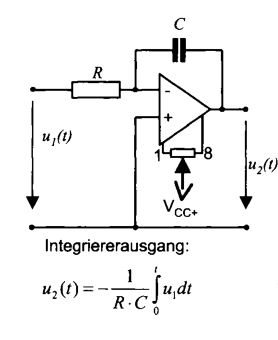
\includegraphics[width=0.4\textwidth]{ANNEX/Fig/AC/AC_06_IntOpamp.JPG}
        \caption{Circuito de un amplificador integrador realiza la función matemática de la integración de la señal de entrada. Extraído de \autocite{libro_aleman}}
        \label{fig:opamp}
        \end{figure}  
        Por otra parte, la constante de generador $k_e$, según la bibliografía consultada, usualmente se asume con un valor cercano o igual al de la constante de par del motor $k_t$. Esta suposición se fundamenta si se desprecia pérdidas de energía por disipación interna (calor) y simplemente se considera que la potencia entre el dominio eléctrico y mecánico será la misma. Según \cite{EcCaracterizacionMotor}, si se desprecia la disipación interna, la potencia convertida cumple la siguiente expresión
        \begin{align}
            P_{m}(t) = P_{R}(t) + P_{L}(t) + P_{u}(t),
            \label{eq:potencia}
        \end{align}
        donde:
        \begin{itemize}
            \item $P_m(t)$ representa la potencia que suministra la fuente que energiza el motor.
            \item $P_R(t)$ es la potencia que disipa la resistencia óhmica del bobinado y las escobillas del motor \ac{DC}.
            \item $P_L(t)$ es la potencia que se disipa en el bobinado interno del motor.
            \item $P_u(t)$ representa la potencia generada por el movimiento del rotor respecto a su eje simétrico.
        \end{itemize}
        Esto se visualiza mejor en la Figura \ref{fig:potencia} a continuación.
        \begin{figure}[H]
        \centering
        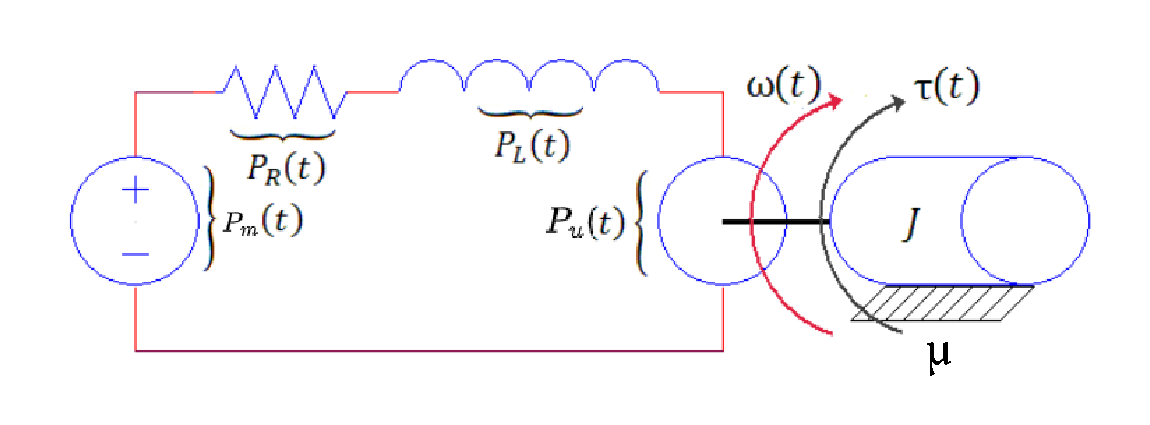
\includegraphics[width=0.65\textwidth]{ANNEX/Fig/AC/AC_07_RelacionPotencia.pdf}
        \caption{Balanceo de potencia del motor \ac{DC}. Adaptado de \autocite{EcCaracterizacionMotor}}
        \label{fig:potencia}
        \end{figure}  
        De la expresión \ref{eq:potencia} se puede reemplazar que la potencia $P_u(t)$ es igual al par del motor $\tau$, el cual, como se define en \ref{eq:CH02_Relaciones_lineales} es la expresión que relaciona el torque con la corriente por medio de la constante de par $k_t$. De modo que
        \begin{align}
            P_{u}(t) & = \tau\,\cdot\omega\\
                     & = K_t\,\cdot i(t)\,\cdot\omega
            \label{eq:pu}
        \end{align}
        Si se reemplazan las expresiones $P_m(t)$, $P_R(t)$ y $P_L(t)$ por las magnitudes que representan y a su vez se reemplaza \ref{eq:pu} en la expresión \ref{eq:potencia} resultaría una ecuación equivalente a la ecuación \ref{eq:ecu_electrica} que modela la parte eléctrica del motor \ac{DC} 
        \begin{align*}
            P_{e}(t) &= u(t)\,i(t) = R\,i(t)^{2} + V_{L}\,i(t) + \omega(t)\,\tau(t)\\
            u(t)\,i(t) &= R\,i(t)^{2} + V_{L}\,i(t) + K_{t}\,i(t)\,\omega(t),
        \end{align*}
        Si se simplifica en cada término la magnitud $i(t)$, el balanceo de potencias resulta exactamente igual a la expresión \ref{eq:ecu_electrica}, que modela el comportamiento eléctrico del sistema de un motor \ac{DC}, con la diferencia que con la expresión
        \begin{align*}
            u(t) &= R\,i(t) + V_{L} + K_{t}\,\omega(t),
        \end{align*}
        se utiliza la constante $k_t$ para la caída de tensión generada por el giro del rotor respecto al eje del motor. Concluyendo así que para que ambas expresiones puedan modelar el mismo fenómeno se debe cumplir que $K_e = K_t$.
        Sin embargo, es usual que los fabricantes que ensamblan los motores \ac{DC}, en las hojas de datos ofrezcan estos parámetros con diferentes unidades. Siendo $k_e$ expresado, como se mencionó al inicio de la presente sección, como $[\mathrm{V\,s/rad}]$, mientras que el parámetro $k_t$ usualmente lo encontramos con unidades de $[\mathrm{Nm/A}]$. Por ello, para guardar la relación dimensional entre estas magnitudes se buscará hallar el factor que compense el trabajar con las mismas magnitudes el cual deberá ser adimensional y lo más pequeño posible para no causar errores por haber asumido la igualdad entre las constantes del motor.
        
        A continuación se muestra el cálculo de ese factor adimensional por parte del autor \cite{EcCaracterizacionMotor} considerando que ambas constantes tendrán de magnitud $[\mathrm{V\,s}]$:
            \begin{align*}
                K_e\,[\mathrm{V\,s\,rad^{-1}}] &= \gamma\,K_t\,[\mathrm{N\,m\,A^{-1}}] \\
                1\,[\mathrm{rad^{-1}}]\;K_e\,[\mathrm{V\,s}] &= \gamma\,K_t\,[\mathrm{J\,A^{-1}}] \\
                1\,[\mathrm{rad^{-1}}]\!\left[\frac{2\pi\,\mathrm{rad}}{\mathrm{rev}}\right]\!K_e\,[\mathrm{V\,s}] &= \gamma\,K_t\,[\mathrm{W\,s\,A^{-1}}] \\
                1\!\left[\frac{2\pi}{\mathrm{rev}}\right]\!K_e\,[\mathrm{V\,s}] &= \gamma\,K_t\,[\mathrm{V\,A\,s\,A^{-1}}] \\
                2\pi\,K_e\,[\mathrm{V\,s}] &= \gamma\,K_t\,[\mathrm{V\,s}] \\
                \gamma &= 2\pi .
            \end{align*}
        
    \subsection{Resistencia de armadura $R$}
    \label{sec:resis}
        Para estimar la resistencia óhmica equivalente $R$ del motor \ac{DC}, se parte de la ecuación eléctrica \eqref{eq:ecu_electrica} y se busca llevarla a la forma de la ley de Ohm midiendo la tensión y la corriente en los terminales del motor. Para ello se inmoviliza el eje aplicando una carga suficientemente grande para impedir el giro al aplicar voltaje. En esta condición de rotor bloqueado, una vez alcanzado el régimen estacionario, se cumple \(\tfrac{di}{dt}\approx 0\) y \(\omega(t)\approx 0\). La primera suposición se asume que la corriente no variará más al no poder vencer el torque que ejerce la carga aplicada en el motor, mientras que la otra suposición la asumiremos debido a que al no existir giro alguno del eje, dicha expresión será igual a cero al no estar generando un voltaje por el giro del eje del motor respecto a su eje concéntrico; así, la ecuación
        \begin{align*}
        u(t) = R\,i(t) + L\,\frac{di}{dt} + K_e\,\omega(t)
        \end{align*} 
        se reduce a
        \begin{align}
        u(t) \approx R\,i(t).
        \end{align}
        De este modo, \(R\) se obtiene a partir de las mediciones como \(R \approx \tfrac{u(t)}{i(t)}\).
        Una recomendación del autor es que se promedie el valor de varias mediciones de la resistencia girando en distintas posiciones del eje del motor. Debido a que, dependiendo de la posición de este, el contacto con las escobillas también variará y, por ende, la resistencia que ejerzan en el sistema también cambiará.
            
    \subsection{Inductancia de armadura $L$}
        De manera análoga a la sección \ref{sec:resis}, se parte de la ecuación eléctrica asumiendo que se le aplicará una carga lo suficientemente grande que haga que el eje del motor no pueda girar. Con el rotor bloqueado se asume que $\omega(t)=0$ y, al ser $u_a(t)=K_e\,\omega(t)$, resulta $u_a(t)=0$. Con esta condición, el circuito tendrá un comportamiento similar al de una malla de circuito en serie $RL$
        \begin{align}
        L\,\frac{di(t)}{dt}+i(t)\,R=\,u(t). 
        \end{align}
        Aplicando un escalón de tensión $u(t)=U_0\,\mathbf{1}(t)$, la corriente del inductor responderá como
        \begin{align}
        i(t)=i_\infty\left(1-e^{-t/t_{63.2\%}}\right),
        \end{align}
        donde $I_\infty=\dfrac{U_0}{R_A}$ es la corriente en estado estacionario y $t_{63.2\%}=\dfrac{L_A}{R_A}$ la constante de tiempo eléctrica.
        
        A partir de la curva de aumento, $t_{63.2\%}$ puede determinarse como el instante en que $i(t)$ alcanza el $63.2\%$ de $I_\infty$. Por tanto, la inductancia se obtiene como        
        \begin{align}
        L_A=R_A\,t_{63.2\%}\,.
        \end{align}
        
    \subsection{Fricción viscosa $\mu$}
        En ausencia de carga externa, el par desarrollado por el motor en régimen compensa únicamente las pérdidas mecánicas por fricción. El modelo clásico se
        expresa como
        \begin{align*}
            \tau_v(\omega)=\tau_c\,\operatorname{sgn}(\omega)+\mu\,\omega,
            \label{eq:ecu_fric}
        \end{align*}
        
        donde $\tau_c$ es el par por deslizamiento (Coulomb) y $\mu$ el coeficiente de
        fricción viscosa.
        
        El par electromagnético se relaciona con la corriente del inducido mediante
        \begin{align*}
        \tau = K_t\,i,
        \end{align*} 
        con $k_t$ mecánica, previamente hallada al asumir el mismo valor de la constante del generador $k_e$. En régimen estacionario y sin carga
        externa se puede simplificar la expresión \ref{eq:ecu_mecanica} a la ecuación
        \begin{align*}
            \tau = \tau_v(\omega) \quad \Longrightarrow \quad K_t\,i(\omega)=\tau_c+\mu\,\omega .
        \end{align*}        
        De aquí se deduce que la fricción total puede identificarse a partir de
        mediciones de corriente y velocidad. Si se realiza un barrido de velocidad (variando la tensión de entrada $v(t)$) y, para cada $\omega$, se registra la corriente $i$ en régimen, la relación anterior predice una dependencia aproximadamente lineal:
        \begin{align*}
            K_t\,i(\omega) \approx \tau_c + \mu\,\omega .
        \end{align*}        
        Despreciando las fricciones estáticas y de Coulomb en el régimen de velocidades bajas, como se menciona en \ref{sec:CH02_ModeloMDC}. Se puede estimar el parámetro de fricción cómo 
        \begin{align}
            K_t\,i = \mu\,\omega .
        \end{align}
        Según \textcite{ModeladoFriccion}, se presenta el modelo completo del componente de fricción a considerar
        \begin{align*}
        \tau_f(\omega)=\underbrace{\tau_s\,\operatorname{sgn}(\omega)}_{\text{estático}}
        +\underbrace{\tau_c\,\operatorname{sgn}(\omega)}_{\text{Coulomb}}
        +\underbrace{\mu\,\omega}_{\text{viscoso}}.  
        \end{align*}
        Sin embargo, para el estudio de este trabajo se considera el modelo simplificado presentado que también es válido. Uno de los resultados de la aproximación tomada en la curva $\tau$–$\omega$ la presenta \textcite{libro_aleman}, donde se muestra que el término viscoso es despreciable y la fricción es esencialmente constante
        (Coulomb) como se muestra en la Figura \ref{fig:friccion}. 
        
        \begin{figure}[H]
        \centering
        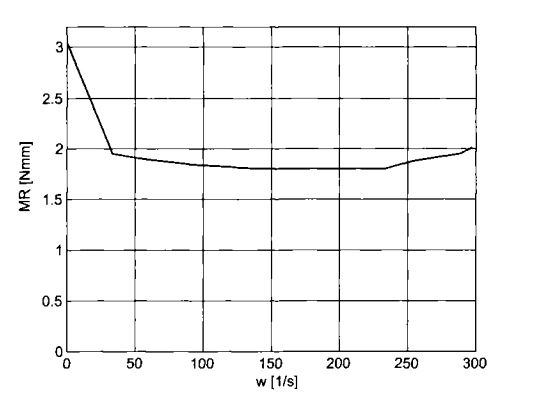
\includegraphics[width=0.6\textwidth]{ANNEX/Fig/AC/AC_08_FriccionViscosa.JPG}
        \caption{Gráfica velocidad–par del motor ($\tau$). Extraído de \textcite{libro_aleman}.}
        \label{fig:friccion}
        \end{figure}
    \subsection{Momento de inercia del rotor $J$}
        En el libro de \textcite{libro_Aleman} se mencionan dos alternativas para determinar el momento de inercia del rotor: una mediante una prueba de vibración y la otra utilizando la medición de la desaceleración del eje del motor.
        En la Figura \ref{fig:rotor_vibracion} se muestra el esquema de análisis para el rotor recortado para pequeñas deflexiones $\phi$ alrededor de la posición de reposo en el centro del eje del rotor.
        \begin{figure}[H]
        \centering
        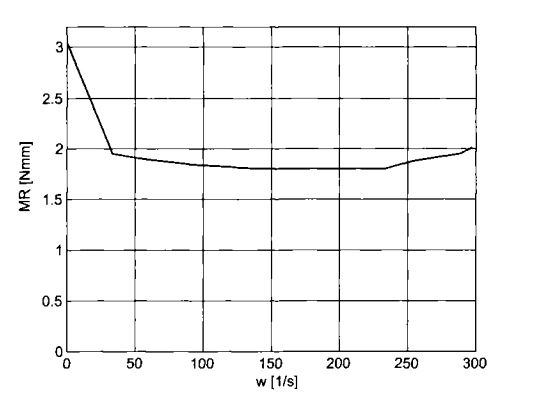
\includegraphics[width=0.6\textwidth]{ANNEX/Fig/AC/AC_08_FriccionViscosa.JPG}
        \caption{Esquema del ensayo para obtener la inercia del rotor. Extraído de \textcite{libro_aleman}.}
        \label{fig:rotor_vibracion}
        \end{figure}
        Este método consiste en colocar una varilla de inercia conocida (en el caso de la Figura \ref{fig:rotor_vibracion} será representada como $J_{st}$), al rotor del motor en uno de sus extremos, mientras que a una distancia $r$ se deberá conectar dos resortes de masa despreciable. Utilizando estos elementos, se procederá a desviar ligeramente la varilla unida al eje del motor y se procederá a medir el periodo de oscilación de esta. Luego de ese experimento, se colocará una masa adicional en el otro extremo de la varilla y se vuelve a realizar la prueba. A partir de la relación entre los dos periodos de oscilación de ambos experimentos se podrá determinar la inercia del rotor con la expresión \ref{eq:rotor} que nace de las siguientes expresiones:
        \begin{align}
        -(J + J_{St})\,\ddot{\varphi} - (F_0 + c\,r\,\varphi)\,r + (F_0 - c\,r\,\varphi)\,r &= 0
        \end{align}
        
        \begin{align}
        \ddot{\varphi} + \frac{c\,r^2}{J + J_{St}}\,\varphi &= 0
        \end{align}
        
        \begin{align}
        \omega_0 = \sqrt{\frac{c\,r^2}{J + J_{St}}} = \frac{2\pi}{T_0}
        \end{align}
        
        \begin{align}
        T_0 = 2\pi \sqrt{\frac{J + J_{St}}{c\,r^2}}
        \end{align}
        
        \begin{align}
        T_1 = 2\pi \sqrt{\frac{J + J_{St} + m\,R^2}{c\,r^2}}
        \end{align}
        
        \begin{align}
        J + J_{St} = \frac{m\,R^2}{\left(\dfrac{T_1}{T_0}\right)^2 - 1}
        \end{align}

        Ecuación mecánica (sin carga externa).
        \[
        J\,\dot\omega + B\,\omega + \tau_c\,\operatorname{sgn}(\omega) = K_t\,i.
        \]
        \label{eq:rotor}
        % Método A (desaceleración libre). Corte la alimentación y registre $\omega(t)$:
        % Si domina fricción viscosa ($\tau_c\approx 0$): $\omega(t)=\omega_0 e^{-(B/J)t}$. De la pendiente en semilog obtiene $B/J$; con $B$ conocido, $J=B/(\text{pendiente})$.
        
\section{Métodos de identificación paramétrica}
    La identificación de sistemas no lineales es un campo que aún se considera relativamente reciente. En aplicaciones mecánicas con motores de corriente continua, este procedimiento se utiliza para analizar y determinar los parámetros del sistema. En los últimos años ha aumentado el interés por la identificación no lineal de motores \ac{DC} y por la compensación de no linealidades presentes, entre ellas la fricción de Coulomb.

    Por otro lado, existen métodos basados en estimadores que automatizan el proceso de extracción de parámetros. En el contexto de 
    Métodos no paramétricos, que permiten obtener modelos no paramétricos del sistema bajo estudio. Algunos de estos métodos son: análisis de la respuesta transitoria, análisis de la respuesta en frecuencia, análisis de la correlación, análisis espectral, análisis de Fourier, etc.
    Métodos paramétricos, que permiten obtener modelos paramétricos. Estos métodos requieren la elección de una posible estructura del modelo, de un criterio de ajuste de parámetros y, por último, de la estimación de los parámetros que mejor ajustan el modelo a los datos experimentales.

    
    % \subsection{Modelos paramétricos para la identificación de sistemas lineales}
    
    % Según la información de \cite{yo cito}, se tienen los siguientes modelos de caja negra basados en polinomios en el operador de retardo \(q^{-1}\).
    
    % \subsubsection*{Modelo ARX}
    % Estructura:
    % \[
    % A(q^{-1})\,y[k] \;=\; q^{-n_k}\,B(q^{-1})\,u[k] \;+\; e[k],
    % \]
    % donde \(A(q^{-1})=1+a_1 q^{-1}+\cdots+a_{n_a}q^{-n_a}\), \(B(q^{-1})=b_0+b_1 q^{-1}+\cdots+b_{n_b}q^{-n_b}\), \(n_k\) es el retardo puro y \(e[k]\) es ruido blanco de predicción. La estimación típica se realiza por mínimos cuadrados o PEM, resultando consistente cuando \(e[k]\) es blanco e independiente de \(u[k]\). Es una estructura simple y con buenos predictores, aunque puede sesgarse si el ruido es coloreado. Véase el esquema en la Figura \ref{fig:YO_ARX}.
    
    % \subsubsection*{Modelo ARMAX}
    % Extiende ARX incorporando un modelo explícito del ruido:
    % \[
    % A(q^{-1})\,y[k] \;=\; q^{-n_k}\,B(q^{-1})\,u[k] \;+\; C(q^{-1})\,e[k],
    % \]
    % con \(C(q^{-1})=1+c_1 q^{-1}+\cdots+c_{n_c}q^{-n_c}\). Al modelar el color del ruido, mejora el desempeño frente a perturbaciones correlacionadas, a costa de una estimación no lineal en los parámetros que suele resolverse con PEM o máxima verosimilitud, usando ARX como inicialización y verificando que los residuos sean aproximadamente blancos. Véase la Figura \ref{fig:YO_ARMAX}.
    
    % \subsubsection*{Modelo entrada–salida (OE)}
    % El modelo entrada–salida representa la planta sin realimentar la salida en el predictor:
    % \[
    % y[k] \;=\; \frac{B(q^{-1})}{F(q^{-1})}\,q^{-n_k}\,u[k] \;+\; e[k],
    % \]
    % donde \(F(q^{-1})=1+f_1 q^{-1}+\cdots+f_{n_f}q^{-n_f}\). Es adecuado cuando el ruido actúa principalmente en la medición de salida y es independiente de la entrada; evita introducir \(A(q^{-1})\) multiplicando a \(y[k]\), lo que reduce sesgos por ruido coloreado respecto a ARX. Véase la Figura \ref{fig:YO_OE}.
    
    % \subsubsection*{Notas comunes}
    % La selección de órdenes \((n_a,n_b,n_c,n_f)\) y del retardo \(n_k\) se apoya en criterios de validación (AIC, BIC, análisis de residuos y capacidad predictiva) y en conocimiento previo del proceso. Para todos los casos, la estimación requiere señales de entrada con excitación suficiente y muestreo acorde con la dinámica del sistema.

    % \subsection{Modelos ARX/ARMAX y algoritmo de Steiglitz--McBride (resumen)}
    
    % Según \cite{yo cito}, para identificar sistemas lineales a partir de datos entrada–salida se emplean modelos polinomiales en el operador de retardo \(q^{-1}\) y criterios de minimización del error de predicción.
    
    % \paragraph{Modelo ARX.}
    % \[
    % A(q^{-1})\,y[k] \;=\; q^{-n_k}\,B(q^{-1})\,u[k] \;+\; e[k],
    % \]
    % con \(A(q^{-1})=1+a_1 q^{-1}+\cdots+a_{n_a}q^{-n_a}\) y \(B(q^{-1})=b_0+b_1 q^{-1}+\cdots+b_{n_b}q^{-n_b}\). Esta estructura posee regresión lineal: la salida estimada se escribe \(y_e[k]=\varphi^\top[k]\theta\), donde \(\varphi[k]\) apila salidas y entradas pasadas, y \(\theta\) contiene \(\{a_i\}\) y \(\{b_j\}\). La estimación por mínimos cuadrados es consistente cuando \(e[k]\) es blanco e independiente de \(u[k]\). Véase la Figura \ref{fig:YO_ARX}.
    
    % \paragraph{Modelo ARMAX.}
    % \[
    % A(q^{-1})\,y[k] \;=\; q^{-n_k}\,B(q^{-1})\,u[k] \;+\; C(q^{-1})\,e[k],
    % \]
    % donde \(C(q^{-1})=1+c_1 q^{-1}+\cdots+c_{n_c}q^{-n_c}\). Al modelar el color del ruido vía \(C(q^{-1})\), reduce sesgos frente a perturbaciones correlacionadas, a costa de una estimación no lineal (típicamente PEM o máxima verosimilitud), usando ARX como inicialización. Véase la Figura \ref{fig:YO_ARMAX}.
    
    % \paragraph{Criterio de ajuste.}
    % El error de predicción \(\varepsilon[k,\theta]=y[k]-y_e[k,\theta]\) se minimiza en media cuadrática sobre un conjunto de datos. La identificación puede ser fuera de línea (post–proceso de un bloque de datos) o en línea (recursiva); aquí se adopta el enfoque fuera de línea \cite{yo cito}.
    
    % \subsubsection*{Algoritmo de Steiglitz--McBride (SM) para ARX}
    
    % El problema directo de minimizar
    % \[
    % \min_{\{a_i,b_j\}}\;\sum_{k}\Bigg[y[k]-\frac{B(q^{-1})}{A(q^{-1})}\,q^{-n_k}u[k]\Bigg]^2
    % \]
    % es no lineal en los parámetros. SM lo transforma en una secuencia de problemas lineales mediante prefiltrado iterativo con el denominador estimado. La idea práctica es:
    
    % \begin{enumerate}
    % \item Inicializar \((A^{(0)},B^{(0)})\) (por ejemplo, con ARX por mínimos cuadrados).
    % \item En la iteración \(t\), construir señales prefiltradas con el denominador anterior:
    % \[
    % \tilde y^{(t)}[k]=\frac{y[k]}{A^{(t-1)}(q^{-1})},\qquad
    % \tilde u^{(t)}[k]=\frac{u[k]}{A^{(t-1)}(q^{-1})}.
    % \]
    % \item Resolver por mínimos cuadrados el modelo lineal en parámetros
    % \[
    % \tilde y^{(t)}[k]\;\approx\; q^{-n_k}\,B^{(t)}(q^{-1})\,\tilde u^{(t)}[k]
    % \;-\;\sum_{i=1}^{n_a} a_i^{(t)}\,\tilde y^{(t)}[k-i],
    % \]
    % obteniendo los nuevos coeficientes \(\{a_i^{(t)},b_j^{(t)}\}\).
    % \item Repetir hasta convergencia o hasta un número prefijado de iteraciones. 
    % \end{enumerate}
    
    % Bajo entrada persistentemente excitante y ruido de medición blanco, el procedimiento converge a estimaciones insesgadas cuando el orden del modelo es suficiente. En la práctica, se verifica la blancura de residuos y la estabilidad del \(A(q^{-1})\); si es necesario, se proyectan los polos dentro del círculo unitario. El flujo de SM puede representarse como en la Figura \ref{fig:YO_SMCB}, donde el primer bloque realiza el prefiltrado \(1/A^{(t-1)}(q^{-1})\) y el segundo resuelve mínimos cuadrados con las señales filtradas \cite{yo cito}.
    
    % \paragraph{Relación con ARMAX y modelos entrada–salida.}
    % SM se formula de forma natural para ARX por su regresión lineal tras el prefiltrado. Para entornos con ruido coloreado, ARMAX modela explícitamente la dinámica del ruido con \(C(q^{-1})\); en ese caso, suele emplearse estimación no lineal (PEM) usando la solución ARX/SM como punto de partida. Cuando el ruido afecta principalmente la salida de medida y se desea evitar realimentar \(y[k]\) en el predictor, puede usarse la estructura entrada–salida \(y[k]=\tfrac{B(q^{-1})}{F(q^{-1})}q^{-n_k}u[k]+e[k]\), estimada típicamente por PEM con inicialización ARX \cite{yo cito}.
    
    % \section{Mínimos Cuadrados (MC): idea, relación con regresión lineal y ecuaciones básicas}
    
    % \textbf{Idea general.} Dados pares de datos $\{(\varphi_k,y_k)\}_{k=1}^N$ y un modelo lineal en parámetros
    % \[
    % y_k \approx \varphi_k^\top \theta,
    % \]
    % MC busca el vector de parámetros $\theta\in\mathbb{R}^p$ que minimiza la suma de cuadrados del error:
    % \[
    % J(\theta)=\sum_{k=1}^N \big(y_k-\varphi_k^\top \theta\big)^2.
    % \]
    % Esto es equivalente a la \textit{regresión lineal} clásica cuando $\varphi_k$ contiene las variables explicativas y $\theta$ son los coeficientes.
    
    % \subsection*{Forma matricial y ecuaciones normales}
    % Defina la matriz de regresores $\Phi\in\mathbb{R}^{N\times p}$ y el vector de salidas $y\in\mathbb{R}^{N}$:
    % \[
    % \Phi=\begin{bmatrix}\varphi_1^\top\\ \varphi_2^\top\\ \vdots\\ \varphi_N^\top\end{bmatrix},\qquad
    % y=\begin{bmatrix}y_1\\ y_2\\ \vdots\\ y_N\end{bmatrix}.
    % \]
    % El criterio es $J(\theta)=\|y-\Phi\theta\|_2^2$. Si $\Phi$ tiene rango columna completo ($\operatorname{rank}(\Phi)=p$), la solución de \textbf{mínimos cuadrados ordinarios (MCO)} es
    % \[
    % \widehat{\theta}_{\text{MCO}}=(\Phi^\top \Phi)^{-1}\Phi^\top y.
    % \]
    % Las \textit{ecuaciones normales} asociadas son
    % \[
    % \Phi^\top \Phi\,\widehat{\theta}=\Phi^\top y.
    % \]
    
    % \subsection*{Versión ponderada (WLS)}
    % Si cada muestra tiene varianza diferente o se desea privilegiar ciertas mediciones, use una matriz de pesos $W=\operatorname{diag}(w_1,\dots,w_N)\succ 0$:
    % \[
    % J(\theta)=\|W^{1/2}(y-\Phi\theta)\|_2^2,\qquad
    % \widehat{\theta}_{\text{WLS}}=(\Phi^\top W \Phi)^{-1}\Phi^\top W y.
    % \]
    
    % \subsection*{Mínimos cuadrados recursivos (RLS)}
    % Para actualizar en línea con nuevas muestras $(\varphi_k,y_k)$:
    % \[
    % \begin{aligned}
    % K_k&=P_{k-1}\varphi_k\big(1+\varphi_k^\top P_{k-1}\varphi_k\big)^{-1},\\
    % \widehat{\theta}_k&=\widehat{\theta}_{k-1}+K_k\big(y_k-\varphi_k^\top \widehat{\theta}_{k-1}\big),\\
    % P_k&=(I-K_k\varphi_k^\top)P_{k-1},
    % \end{aligned}
    % \]
    % con condiciones iniciales $\widehat{\theta}_0$ y $P_0\succ 0$. Un factor de \textit{olvido} $\lambda\in(0,1]$ se incorpora reemplazando $1$ por $\lambda$ en el denominador de $K_k$.
    
    % \subsection*{Relación con regresión lineal}
    % La regresión lineal clásica asume $y=\Phi\theta+\varepsilon$ con $\varepsilon\sim\mathcal{N}(0,\sigma^2 I)$. Bajo esas hipótesis, MCO es insesgado y de varianza mínima entre estimadores lineales insesgados (teorema de Gauss–Markov). La matriz de covarianza de $\widehat{\theta}$ (si $\sigma^2$ es conocida) es
    % \[
    % \operatorname{Cov}(\widehat{\theta})=\sigma^2(\Phi^\top\Phi)^{-1}.
    % \]